% !TEX TS-program = pdflatex
% !TEX encoding = UTF-8 Unicode

% This is a simple template for a LaTeX document using the "article" class.
% See "book", "report", "letter" for other types of document.

\documentclass[11pt]{article} % use larger type; default would be 10pt

\usepackage[utf8]{inputenc} % set input encoding (not needed with XeLaTeX)

%%% Examples of Article customizations
% These packages are optional, depending whether you want the features they provide.
% See the LaTeX Companion or other references for full information.

%%% PAGE DIMENSIONS
\usepackage{geometry} % to change the page dimensions
\geometry{a4paper} % or letterpaper (US) or a5paper or....
% \geometry{margins=2in} % for example, change the margins to 2 inches all round
% \geometry{landscape} % set up the page for landscape
%   read geometry.pdf for detailed page layout information

%%% Line Spacing
\usepackage{setspace}
\onehalfspacing

\usepackage{graphicx} % support the \includegraphics command and options

% \usepackage[parfill]{parskip} % Activate to begin paragraphs with an empty line rather than an indent

%%% PACKAGES
\usepackage{booktabs} % for much better looking tables
\usepackage{array} % for better arrays (eg matrices) in maths
\usepackage{verbatim} % adds environment for commenting out blocks of text & for better verbatim
\usepackage{subfig} % make it possible to include more than one captioned figure/table in a single float
\usepackage{amsmath, amssymb, amsthm, lastpage}
% These packages are all incorporated in the memoir class to one degree or another...

%%% HEADERS & FOOTERS
\usepackage{fancyhdr} % This should be set AFTER setting up the page geometry
\pagestyle{fancy} % options: empty , plain , fancy
\renewcommand{\headrulewidth}{0pt} % customise the layout...
\lhead{Team \# 16677}\chead{}\rhead{Page \thepage\ of \pageref{LastPage}}
\lfoot{}\rfoot{}\cfoot{}

%%% SECTION TITLE APPEARANCE
%\usepackage{sectsty}
%\allsectionsfont{\sffamily\mdseries\upshape} % (See the fntguide.pdf for font help)
% (This matches ConTeXt defaults)

%%% ToC (table of contents) APPEARANCE
%\usepackage[nottoc,notlof,notlot]{tocbibind} % Put the bibliography in the ToC
%\usepackage[titles,subfigure]{tocloft} % Alter the style of the Table of Contents
%\renewcommand{\cftsecfont}{\rmfamily\mdseries\upshape}
%\renewcommand{\cftsecpagefont}{\rmfamily\mdseries\upshape} % No bold!

%%% END Article customizations

%%% The "real" document content comes below...
%\date{}

\begin{document}
\begin{titlepage}
    \vspace*{\fill}
    \begin{center}
      \Huge{Where's my Ferry?}\\[0.5cm]
      \Large{Support Vector Machines for Modeling Ferry Tardiness}\\[0.4cm]
      \today
    \end{center}
    \vspace*{\fill}
  \end{titlepage}
\newpage
\vspace*{\fill}
\tableofcontents
\vspace*{\fill}
\newpage

\section{Introduction}
\label{sec:intro}
Ferries (as in \textbf{Figure~\ref{fig:basicferry}} present an interesting 
opportunity to examine a complex traffic system filled with data and affecting 
the lives of many individuals. This paper will discuss a new approach to predicting 
the timeliness of ferries using a support vector machine.  An overview of how 
support vector machines work and their complications in real world use will 
introduce the discussion of how this powerful construct presents a powerful and 
intuitive model for tackling the massive data associated with ferries.  A 
functioning model is developed to examine the complexities of this
approach, the practicality, and as a means of exploring some of the data.

\begin{figure}[h]
  \centering
  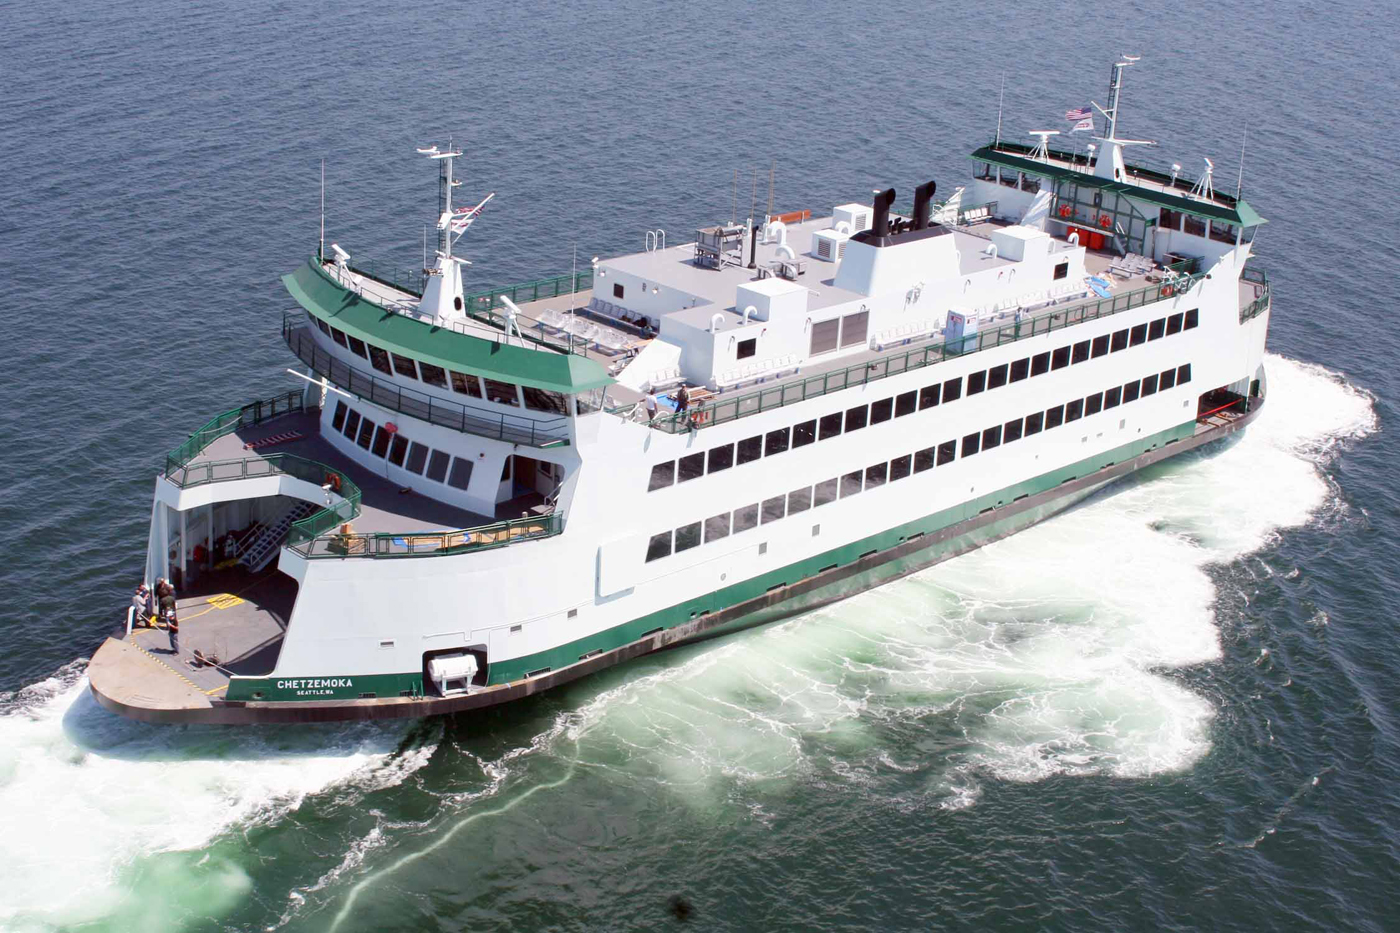
\includegraphics[scale=.15]{images/ferry.jpg}
  \caption{A prototypical WSDOT ferry on its route.}
  \label{fig:basicferry}
\end{figure}

We will attempt to predict the tardiness of ferries, where tardy is 
defined as no less than three minutes later than the
initial (at day's beginning) scheduled arrival or departure time. This definition
of tardiness was chosen to allow for a non-trivial number of tardy events 
(more than 10% in the data) and to remain practical: i.e. someone could use the
restroom in three minutes time or otherwise make use of that information. The 
Washington State Department of Transportation's ferry system in the Pacific
Northwest served as the source for all data. As will be discussed later on, 
this ferry system is notoriously on time with over 95\% of trips being on 
schedule (within one minute). %TODO: CITATION
This system is of particular interest for its sheer volume of passengers: 
22 million per year. %TODO:CITATION
The volume lends itself well to this project's goals of using data mining. 
% TODO: better transition sentence is needed



\section{Preliminaries}
\label{sec:prelims}
Since the goal of the project was to use a large data set for machine learning 
and to develop a model for possibly predict future ferry tardiness, two approaches
popular in available implementations and the literature were initially evaluated:
artificial neural networks (ANN) and support vector machines (SVM). These two 
approaches fit into the
category of \textbf{supervised learning}: labeled (known) data is fed into an
algorithm that learns to make better predictions through comparing its own 
predictions to the labeled data set. ANN and SVM are often considered to be
very similar in the problems they attempt to tackle, especially since each can
be used as a linear classifier: a function taking in some object and determining 
a class to which it belongs. Rather than considering tardiness as a spectrum of
degrees, we approach tardiness as a binary feature: late or not. This conceptually
simplifies our problem.  
% TODO: Discuss airlines tardiness example as a motivator for choosing SVM
% and formulating problem as classification
If artificial neural networks and support vector 
machines can both solve classification problems, however, which are we supposed
to choose?

Byvatov et al examine the differences of the two approaches for classifying drugs
\cite{byvatov2003comparison}. While their model certainly isn't for a ferry 
system, their discussion suggests data sets with many features (an aspect of the 
ferry model we discuss later) are better suited for SVM, and they also find little
difference in the predictions of ANN and SVM. Most importantly, their conclusion,
and that of their references, is the two approaches are complementary. Each 
tool catches different cases, but the results are comparable in each approach,
and SVM may even require less ``tweaking''.

Support vector machines are also more intuitively motivated. Consider mapping the
features of a ferry trip (time of departure, weather, boat name, etc.) into a
coordinate plane.  Now, if we do this for all the points in our training set,
we can also attach labels to the points (late or not, as in 
\textbf{Figure~\ref{fig:basic_svm_data}}). In two dimensions, we
could try drawing a line through the late and not-late points to separate them.
This line is simply a hyperplane in higher dimensions, and SVM has its theoretical
underpinnings based on the idea of drawing this hyperplane optimally. In 
\textbf{Figure~\ref{fig:training_hyperplanes}}, we show a sample training of a 
simple support vector machine.

\begin{figure}[h]
  \centering
  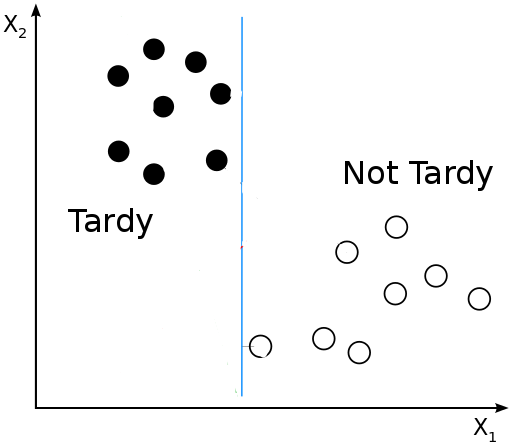
\includegraphics[scale=.5]{images/basic_svm_data.png}
  \caption{A simple example of a separating line for tardiness (i.e. hyperplane). 
      Each data point (or instance) has features $X_1$ and $X_2$.}
  \label{fig:basic_svm_data}
\end{figure}

\begin{figure}[h]
  \centering
  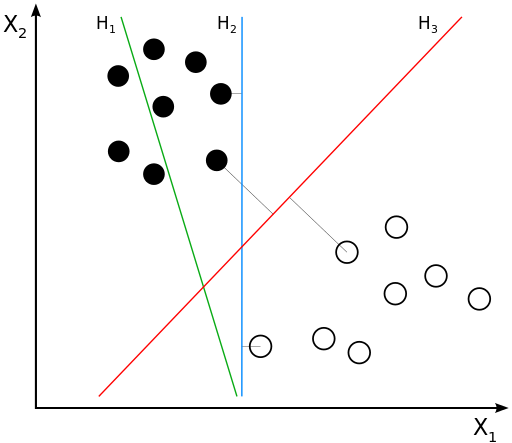
\includegraphics[scale=.5]{images/Svm_separating_hyperplanes.png}
  \caption{As in \textbf{Figure~\ref{fig:basic_svm_data}}, we are trying to separate
    labeled points with a line. A SVM does this iteratively, meaning line $H_1$
    would be the first pass, $H_2$ the result of refitting, and $H_3$ the final 
    classifier produced by the SVM.}
  \label{fig:training_hyperplanes}
\end{figure}

SVM are used as the tool for finding a linear classifier in this project mostly
for ease of understanding and the possibility for use in regression analysis
(a topic discussed in \cite{chang2011libsvm}). 
% TODO: Finalize by leading into a quick discussion of how the SVM algorithm
% works and kernels (or just kernels)


% All the parts of a good time 
% Hyperplanes
% Ferries
% Big (messy) data
% Tardiness
% 
% This is an introduction slide.  I just need to quickly go over
%  who I worked with, that I wanted to learn about AI in practical 
%  situations and do something real with real data, what my project 
%  was (Senior Project/Thesis), what's the problem, and what my 
%  solution was.

% TODO: Possibly include some comparisons of our model to existing research if any.
% Classification as a model
% Tardy or not
% Features are intuitive
%  Route
%  Vessel
%  Weather
% Hyperplanes are (mostly) intuitive
%

\subsection{SVMs for tardiness}
\label{sec:svms_tardiness}
  
% Discuss the major benefits of SVM for my project: features, 
%  the drawing analogy, use for big data. 
% 
% Common uses of classification
%  Spam
%  Cancer
%  Facial recognition
%  Airplane traffic
%  <img style="float:right;margin:4px;"width="50%" height="50%" 
%  src="images/male-female.png">
%  
%  (email, cancer pictures, use in a paper regarding 
%  airlines) 
% 
%  A 2008 paper discussed the use of SVM for predicting a sort of 
%  "bad day" for air traffic control (weather based mostly).  
%  78\% accurate on predicting need to use some sort of software 
%  and 83\% for predicting delays in air traffic.  They used a 
%  super computer.
% 
%  ## Ho! An example!
%  <img src="images/basic_svm_data.png">
%  2. What an SVM is
%      1. How an SVM works
%      2. How it relates to the ferry problem
%          1. Separating late as >3 minutes past estimate
%          2. The data as points in >33 space
%      3. The complication of fitting such a curve
% 
% 

\subsection{Linear classifiers}
\label{sec:lcs}
%  ## Linear classifiers
%  * Feature vector
%  * Weight vector (line, plane, hyperplane)
%  * Sign of dot product is the "class"
% /script>
% /section>
% 

\subsubsection{Feature vectors}
\label{sec:feature_vecs}
%  ## Feature Vectors
%       Time (seconds),
%       Humidity (percent),
%       Temperature (F),
%       Wind Speed (mph),
%       Wind Direction (degrees off N),
%       Vessel Name,
%       Route Name
% 
%       360
%       10,
%       3,
%       6,
%       17,
%       USS Enterprise,
%       Pt. D/Tahlequah
% 
%  Two of these are not like the others.
% 
%  ## Categorical to numeric
%      USS Enterprise,
%      S.S. Minnow,
%      Millenium Falcon,
%      Death Star
%  
%  An average trip for Han Solo:
% 
%      0,
%      0,
%      1,
%      0
% 
% ## WOAH! 
%  ## How do we get the weights?
% 

\subsubsection{Training}
\label{sec:training}
%  ## Learning with </br>Support Vector Machines 
%  * Training data
%    - Mix of both classes
%    - "Big"
%  * A machine to train the weight vector
%    - Draws those lines many times
%    - Knows when to stop
%  * Mighty hardware to do the calculations
%    - Exponentially difficult
%    - Long running process
% 

%  ## How will we know it works?
%  ### Test data for validation
%  - Disjoint from training data
%  - Mix of both classes
%  - Also "big"
% 

%  ## Visualizing an SVM
%  <img src="images/Svm_separating_hyperplanes.png">
%  2. What an SVM is
%      1. How an SVM works
%      2. How it relates to the ferry problem
%          1. Separating late as >3 minutes past estimate
%          2. The data as points in >33 space
%      3. The complication of fitting such a curve
% 
% 
%  ## A real world problem:
%  <img width="50%" height="50%" src="images/tough-separation.png">
% 

\subsubsection{Kernels}
\label{sec:kernels}
%  ## Kernels: bending space
%  <img src="images/kernel-machine.png">
% 
%  ## Tuning the kernel
%  <img src="images/grid_search.png">
%  Like a brute force search
%  Try many (almost all) possibilities
%  Need to bound it
%  Use model accuracy as a performance metric
%  Measured through cross validation
% 

\subsection{LibSVM}
\label{sec:libsvm}
%  ## LibSVM
%  Chih-Chung Chang and Chih-Jen Lin
% 
%  "Working set selection using second 
%  </br>order information for training SVM"
% 
%  <image height="40%" width="40%" src="images/chih-jen.gif">
%  3. Use of LibSVM
%      1. Why not write my own?
%          1. Time
%          2. Correctness
%          3. Performance
%      2. Use in other papers/popularity
%      3. Ease of use of the library (reasonably documented)
%


\section{The problem with ferries}
\label{sec:problem}
%    ## Why do we care about ferries?
%    ### <p class="fragment roll-in">Popular</p>
%    ### <p class="fragment roll-in">Complex</p>
%    ### <p class="fragment roll-in">Lots of data</p>
%    Talk about what the ferry system is (WSDOT), 
%    and how many people use it, how the problem 
%    extends.
% 

\subsection{Washington State's ferries}
\label{sec:wsdot}
%  A portrait of the system</h2>
%       Established in 1951</li>
%        22 million passengers per year</li>
%        20 terminals, 10 routes, 23 vessels</li>
%        Largest ferry system in the world for vehicles</li>
%        From Victoria to Pt. Defiance (~130 miles)</li>
%        159,811 sailings in 2012 (12,764 in December)</li>
%        Almost 10,000,000 vehicles in 2011</li>
%     <img width="110%" 
%      src="images/route-map-overview.gif" align="right">
%  Go over the details of the ferry system.
%  1. history
%  1. Boats
%  2. # Of trips per day
%  3. Routes
%  4. Places serviced
%  6. Design and planning
%  7. Resources for travelers
%    1. Vessel Watch
%    2. Pamphlets
%    3. General knowledge
%    4. Email alerts
%  * Mention that ~95% of boats are on time.  This poses some interesting
%    questions about what we can actually learn.
% 
%  96.4% on time 
%  Best: Pt. Defiance/Tahlequah and Edmonds/Kingston (99.5%)
%  Worst: Anacortes/San Juans (88.9%)
% 

\subsection{Where the data comes from}
\label{sec:data_origins}
%  ## Sources and shades of data
%  * <p class="fragment roll-in">Scraping web pages</p>
%  * <p class="fragment roll-in">WSDOT VesselWatch</p>
%  * <p class="fragment roll-in">NOAA Tacoma Narrows weather station</p>
%  <img src="images/vesselwatch.png">
%  1. Accessibility of the Vessel Watch data
%      1. Briefly discuss the web page scraper
%          1. Using a simulated web browser
%          2. Accounting for "botched" grabs
%      2. Using a request for the data
%          1. Discuss what I actually received
%          2. Discuss the quality and amount of data
%  2. Grabbing weather data
%      1. Grabbed from a deeply hidden NOAA archive
%      2. Manually downloaded files
%      3. Why the Tacoma Narrows station
%          1. Completeness of dates
%          2. Completeness of records
% 
%  ## Ferry data (340,902)
%      Kittitas, Mukilteo, Clinton, 9/1/2010 0:00, 9/1/2010 0:01,
%      Mukilteo - Clinton, 9/1/2010 0:13, 9/1/2010 0:14, 9/1/2010
% 
%  </br>
%  ## Weather data (1184 &times; 24)
%      94274,20110101,0053,12,CLR, ,10.00, , , ,25, ,-3.9, ,22, ,-5.4, ,
%      16, ,-8.9, , 69, , 0, ,000, , , ,29.69, ,1, ,002, ,30.04, ,AA, , ,
%      ,30.03, 
% 
%  ## Weather variables 
% 
% talk about the many weather variables I got from NOAA.
% 
%  ## Data monsters 
%    * Python for everything
%    * 1,034 weather recordings missing wind data
%    * 13,220 vessel trips removed from lack of weather data (~ 4%)
%    * Stages of formatting
%        - Combine all weather data files from NOAA
%        - Join ferry and weather data
%        - Handle categorical variables
%        - Make it all SVMable
%  1. Discussion of data quality
%    1. Missing values
%    2. Ill formatted values
%    3. Generally consistent (huge amount so a few mistakes is okay)
%  2. Separated into 290,000 for training and 30,000 for testing
%  2. Suite of Python scripts to cut out bad data
%  3. Scripts to join weather and ferry data
%  4. Performance issues encountered
% 

%  ## Goal refresh 
%  * Find order in the mess: Which features matter?
%  * Do something practical: Can we use the model?
%  * Work with big data: Was all of the data necessary/useful?
% 90 accuracy isn't expected!  This would be weird in most cases.
% This is because it can't be perfect, there is a maximum iter 
% threshold, it's optimization, noise is still noise, 
% 
% Mention the 95% accurate fact and how we can basically be correct
% Most of the time by guessing on time.  We want a model to be similarly
% accurate.
% 

\subsection{The first pass}
\label{sec:firstpass}
%  ## SVM is easy right?
%  # <p class="fragment roll-in">No. 60%</p>
%  WHY DID I DO BETTER???
%  1. Accuracy comes from test data (disjoint from train data)
%  1. Needing to fit c and gamma parameters to get better curves
%  2. Duration of runs and sheer size of data sets
% 

\subsection{General results}
\label{sec:results}
%  ## Results: Arrivals
%  *  Full: 87.0%
%  *  No Weather: 88.0%
%  *  No Departure: 60.0%
%  *  No Departure, No Weather: 59.4%
%  Full = Departure estimate and actual,
%  arrival estimate, vessel name, route, all weather
%  1. How do we know it's correct?
%      1. Classification versus regression: I want a "useful" machine
%      2. Test sets vs. training sets
%  2. Review the numbers of the results
%      1. Results before param fitting of c and gamma
%      1. Departures
%          1. Weather
%          2. No weather
%      2. The more interesting: arrivals
%          1. Weather
%          2. No weather
% 
%  ## Results: Departures
%  * Full: 76.3%
%  * No Weather: 75.7%
%  Full = Departure estimate, vessel name, route, all weather
% 
%       <img width="70%" src="images/route-map-overview.gif" align="right">

\subsection{The problem with weather}
\label{sec:weather_prob}
% ## How about that weather?
%  Weather/No Weather
% Without information about the departure, the arrival time
%    predictions were strictly less than 68% accuracy.
%  1. Possible issues
%      1. Location of station
%      2. Poor quality of data
%      3. My error
%      4. Ferries really are consistent enough to not need weather
%  2. Running individual routes
%      1. Closest to Tacoma Narrows
%      2. Middleish (randomly selected)
%      3. Geographically furthest

% TODO: Add in the actual weather data to discuss

\section{Closing thoughts}
\label{sec:summary}
%  ## In summary
%  * This is a "cute" model.
%  * Hyperplanes are more than an awesome word.
%  * The ferry system is full of data we can mine.
%  * SVM is like a black box.
% 

\subsection{Remaining questions}
\label{sec:questions}
%  1. Making an actual application
%      1. State of Java web frameworks
%      2. Need to scrape or grab user data
%      3. Update SVM
%  2. Are the schedules online adjusted as time goes by
%  3. Mining the data for patterns
% 

\subsection{Extensions}
\label{sec:extensions}
%  ## Future(ish) work
%  * Multi-class SVM for "tardiness categories"
%  * Regression analysis
%  * Graphical application


\newpage 

\bibliographystyle{amsplain}
\bibliography{undergraduate-thesis.bib}

\end{document}

